\documentclass[11pt,a4paper]{article}
\usepackage{times}
\usepackage{geometry}
\usepackage{graphicx}
\usepackage{amsmath, amssymb}
\usepackage{float}
\usepackage{booktabs}
\usepackage{hyperref}
\hypersetup{hidelinks}
\usepackage{setspace}
\usepackage{caption}

\geometry{margin=1in}
%\onehalfspacing

\title{
\textbf{\Large Embedding-Free Approaches to Sentiment Classification:\\
A comparative study on Instagram comments}
}

\author{
Mandira Majhi, MD2414 \quad
Manopriya Pal, MD2415 \\
Bishwayan Ghosh, MD2405 \quad
Baidurya Bhattacharyya, MD2403 \\
\normalsize Indian Statistical Institute
}

\date{\today}

\begin{document}

\maketitle

\begin{abstract}
Instagram comments are short, noisy, and highly informal, yet they exhibit rich emotional cues that make them suitable for sentiment classification tasks. This project presents a systematic pattern recognition study on a manually curated dataset of 1333 Instagram comments, each labelled into one of three sentiment categories. After constructing a robust preprocessing pipeline to clean and standardise the text, we evaluate a suite of classical machine learning models—Logistic Regression, Support Vector Machines, Multinomial Naive Bayes, and XGBoost—alongside a fine-tuned DistilBERT transformer. Our results show that while linear models provide strong and interpretable baselines on sparse lexical features, DistilBERT achieves the highest overall performance due to its ability to capture deeper contextual cues in informal comment text. We further explore a context-free formulation of the task, removing video descriptions to simulate real-world deployment conditions, and observe that model performance remains largely stable. The study highlights the practicality of lightweight linear models and the superior accuracy of transformer-based approaches, offering insights into scalable sentiment analysis for social-media environments.
\end{abstract}

\tableofcontents

% ============================================================
\section{Introduction}
The rapid growth of social media has transformed the landscape of communication. Platforms such as Instagram host millions of interactions per minute, with comments often expressing emotions, opinions, humour, or hostility. Automatically identifying the sentiment of these comments---here in three discrete classes---is a canonical pattern recognition problem combining text processing, statistical modelling, and machine learning.

Sentiment analysis belongs to the broader domain of Natural Language Processing (NLP). While earlier systems relied on lexicons and rule-based heuristics, contemporary approaches emphasise data-driven statistical modelling, including neural architectures capable of capturing long-range linguistic dependencies.

This project focuses specifically on Instagram comments due to their informal tone, prevalence of slang, emojis, and inconsistent punctuation, all of which pose substantial modelling challenges.

\vspace{0.5em}
\subsection*{Objectives:}
\begin{itemize}
    \item Construct a labelled sentiment dataset of Instagram comments (three-class classification).
    \item Perform rigorous text preprocessing and representation.
    \item Train and evaluate classical and neural models.
    \item Compare model performance and articulate findings.
\end{itemize}


% ============================================================
\section{Related Work}
Sentiment analysis has been widely studied across domains, from product reviews to political discourse. Early works applied Naive Bayes and SVMs using bag-of-words (BoW) or TF-IDF vectors. The advent of distributed representations such as Word2Vec and GloVe provided dense embeddings capturing semantic relationships.

Recurrent neural networks, especially LSTMs, extended modelling capability to sequential text. Recently, transformer-based architectures such as BERT and RoBERTa have achieved state-of-the-art performance through bidirectional attention and pretraining on large corpora. However, their performance on short, noisy, highly informal comment text remains an open empirical question, motivating experiments tailored to the Instagram domain.


% ============================================================
\section{Dataset Description}
The dataset consists of \textbf{1333 Instagram comments} with \textbf{manually assigned sentiment labels} in \textbf{3 categories}. Each entry contains the \textbf{context} summarizing what the video is about, the \textbf{raw text comment} and its \textbf{target sentiment class}.

\begin{figure}[H]
\centering
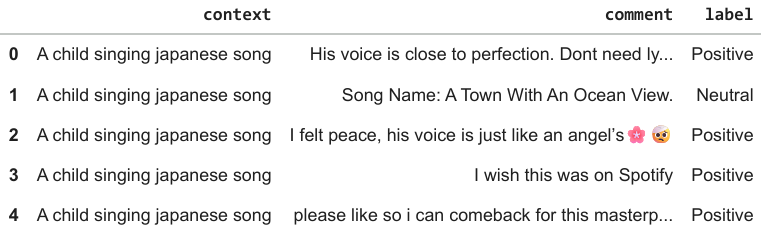
\includegraphics[width=0.6\linewidth]{dataset.png}
\caption{A glimpse of the dataset.}
\end{figure}

\subsection{Characteristics}
\begin{itemize}
    \item Short comment length (most under 15 tokens).
    \item Frequent use of emojis and slang.
    \item Limited grammatical structure.
    \item Presence of domain-specific markers (hashtags, mentions).
\end{itemize}

\subsection{Label Distribution}
A labelled histogram from the report indicates slight class imbalance, though not severe enough to require resampling.

\begin{figure}[H]
\centering
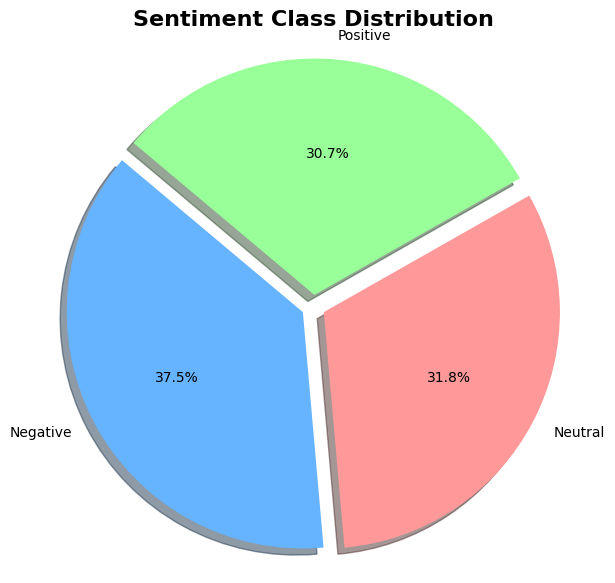
\includegraphics[width=0.5\linewidth]{class-dist-pie.png}
\caption{Dataset class distribution.}
\end{figure}
\begin{figure}[H]
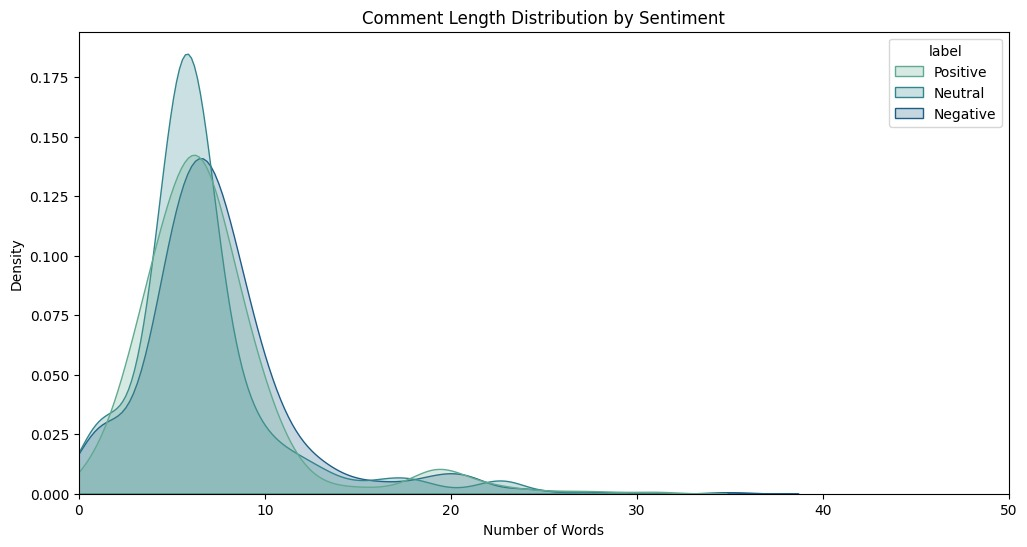
\includegraphics[width=1\linewidth]{comment-length.jpg}
\caption{Classwise comment length distribution.}
\end{figure}


% ============================================================
\section{Preprocessing Pipeline}
Preprocessing was performed systematically to reduce noise and standardize the text while retaining semantic cues.


\subsection*{Steps}
\begin{enumerate}
    \item Lowercasing text.
    \item Eliminating punctuation and special characters except ! and ?
    \item Converting emoji's to their text labels.    
    \item Tokenization using standard word-level tokenizers: Count-vectorizer.
    \item Removal of custom-stopwords: This is an important step for statistical models, more so than neural models. Standard stop-word removal will not work
    \item Lemmatization: Conversion of alternate-forms into their base-forms.
\end{enumerate}

\begin{figure}[H]
    \centering
    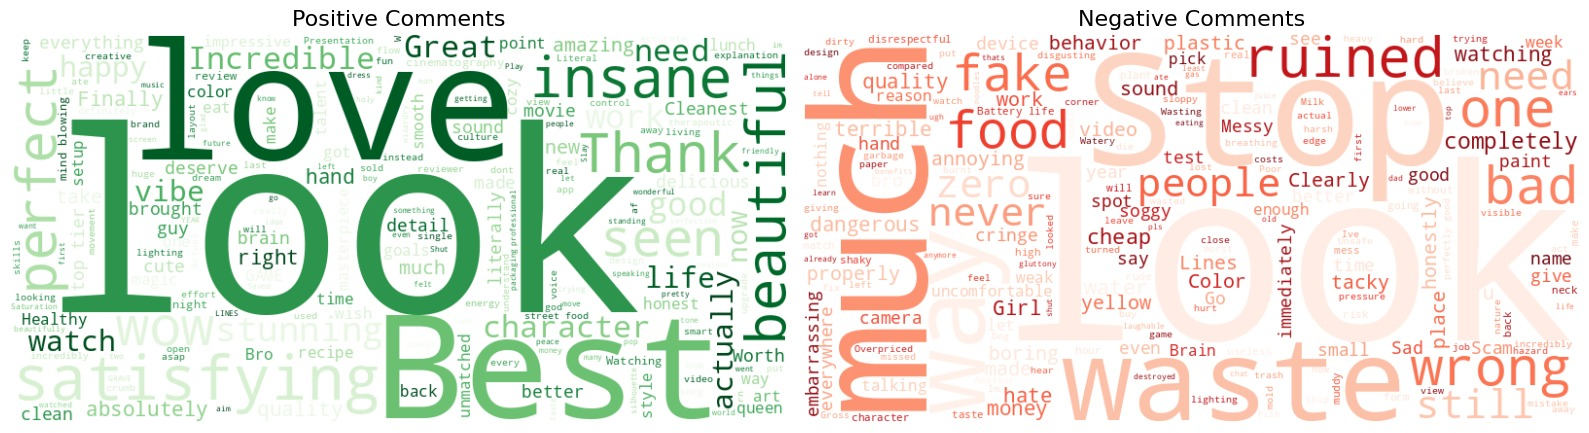
\includegraphics[width=0.9\linewidth]{image.png}
    \caption{Word Clouds of Positive and Negative Classes}
    \label{fig:placeholder}
\end{figure}




% ============================================================

\section*{Model Descriptions}
A diverse set of classifiers was explored.
% OPTION 1: Using an Itemize list (Good for "Methodology" sections)
\begin{itemize}
    \item \textbf{Na\"ive Bayes Classifier:} 
    A probabilistic classifier based on Bayes' theorem that assumes independence between features. To process text, it typically uses a \texttt{CountVectorizer} to convert raw documents into numerical feature vectors $\mathbf{x} = (x_1, \dots, x_n)$ representing word frequencies (Bag-of-Words). It calculates the posterior probability as:
    \begin{equation}
        \hat{y} = \operatorname*{argmax}_{y} P(y) \prod_{i=1}^{n} P(x_i | y)
    \end{equation}
    where $P(y)$ is the prior probability and $P(x_i | y)$ is the likelihood of feature $x_i$ appearing in class $y$. \\

    \item \textbf{Logistic Regression:}
    A linear model used for binary classification that estimates the probability that a given input point belongs to a certain class. Like Na\"ive Bayes, it operates on numerical feature vectors $\mathbf{x}$ generated by \texttt{CountVectorizer}. The model applies the logistic sigmoid function to a linear combination of inputs:
    \begin{equation}
        P(y=1 | \mathbf{x}) = \sigma(\mathbf{w}^T \mathbf{x} + b) = \frac{1}{1 + e^{-(\mathbf{w}^T \mathbf{x} + b)}}
    \end{equation}
    where $\mathbf{w}$ is the weight vector and $b$ is the bias term. The model parameters are estimated by minimizing the log-loss (cross-entropy) function. \\

    \item \textbf{Support Vector Machine (SVM):} 
    A discriminative classifier that finds the optimal hyperplane which maximizes the margin between classes. Like Na\"ive Bayes, it requires text to be vectorized (e.g., via \texttt{CountVectorizer} or TF-IDF) into numerical input vectors $\mathbf{x}_i$. The optimization objective is:
    \begin{equation}
        \min_{\mathbf{w}, b} \frac{1}{2} ||\mathbf{w}||^2 + C \sum_{i=1}^{N} \max(0, 1 - y_i(\mathbf{w}^T \mathbf{x}_i + b))
    \end{equation}
    where $\mathbf{w}$ is the weight vector, $b$ is the bias, and $C$ is the regularization parameter controlling the trade-off between margin maximization and classification error. \\

    \item \textbf{XGBoost (Extreme Gradient Boosting):}
    An efficient and scalable implementation of gradient boosting that builds an ensemble of weak prediction models (decision trees). It operates on numerical matrices generated by \texttt{CountVectorizer}. The model minimizes a regularized objective function:
    \begin{equation}
        \mathcal{L}(\phi) = \sum_{i} l(\hat{y}_i, y_i) + \sum_{k} \Omega(f_k)
    \end{equation}
    where $l$ is a differentiable convex loss function measuring the difference between the prediction $\hat{y}_i$ and the target $y_i$, and $\Omega(f_k)$ penalizes the complexity of the trees to prevent overfitting. \\

    \item \textbf{DistilBERT (Transformer Model):} 
    A distilled version of the BERT model that utilizes self-attention mechanisms. Unlike traditional models, it relies on a specific \texttt{AutoTokenizer} to handle subword tokenization, mapping text to the model's vocabulary and generating special tokens (CLS, SEP).\\
\begin{itemize}
    \item \texttt{[CLS]} (Classification Token): A special token prepended to the start of every sequence; its final hidden vector is used as the aggregate representation of the entire text for classification tasks.
    \item \texttt{[SEP]} (Separator Token): A special marker used to delimit the end of a sentence or separate two different segments of text (e.g., in question-answering pairs).
\end{itemize}

The core attention mechanism is defined as:
    \begin{equation}
        \text{Attention}(Q, K, V) = \text{softmax}\left(\frac{QK^T}{\sqrt{d_k}}\right)V
    \end{equation}
    where $Q$, $K$, and $V$ represent the Query, Key, and Value matrices derived from the tokenized inputs, and $d_k$ is the scaling factor.
\end{itemize}
% ============================================================
\section{Experimental Setup}
\subsection{Train-Test Split}
A standard 75--25 train-test split was used, stratified by sentiment class.
\subsection*{Evaluation Metrics}

\begin{itemize}
    \item \textbf{Accuracy:} 
    The ratio of correctly predicted observations to the total observations. It provides a general measure of the model's performance across all classes but can be misleading if the dataset is imbalanced.
    \begin{equation}
        \text{Accuracy} = \frac{\text{True Positives} + \text{True Negatives}}{\text{Total Samples}}
    \end{equation}

    \item \textbf{Precision (Positive Predictive Value):} 
    The ratio of correctly predicted positive observations to the total predicted positives. It indicates how reliable the model is when it claims a comment is ``Positive.'' High precision means low false positive rate.
    \begin{equation}
        \text{Precision} = \frac{\text{True Positives}}{\text{True Positives} + \text{False Positives}}
    \end{equation}

    \item \textbf{Recall (Sensitivity):} 
    The ratio of correctly predicted positive observations to the all observations in the actual class. It measures the model's ability to find all the positive comments in the dataset.
    \begin{equation}
        \text{Recall} = \frac{\text{True Positives}}{\text{True Positives} + \text{False Negatives}}
    \end{equation}

    \item \textbf{F1-Score:} 
    The weighted average (harmonic mean) of Precision and Recall. It is particularly useful when you need to balance precision and recall, or when there is an uneven class distribution.
    \begin{equation}
        \text{F1-Score} = 2 \times \frac{\text{Precision} \times \text{Recall}}{\text{Precision} + \text{Recall}}
    \end{equation}

    \item \textbf{Confusion Matrix:} 
    A table that visualizes the performance of the algorithm by comparing the actual target values with those predicted by the machine learning model. It breaks down results into True Positives (TP), True Negatives (TN), False Positives (FP), and False Negatives (FN).
\end{itemize}

% ============================================================
\section{Results}
The following performance trends were observed:

\subsection{Statistical Models}
\begin{itemize}
    \item SVM performed strongly, capturing discriminative lexical patterns.
    \item Logistic regression showed competitive but slightly lower accuracy.
\end{itemize}

\subsection{Neural Models}
\begin{itemize}
    \item Transformers achieved the highest overall accuracy due to contextual understanding, despite the short comment length.
\end{itemize}

Performances of different models over the test sets are compared in Figures 5 (Confusion Matrices), 6 (Classwise Recalls) and 7 (F1 Scores).

\begin{figure}[H]
\centering
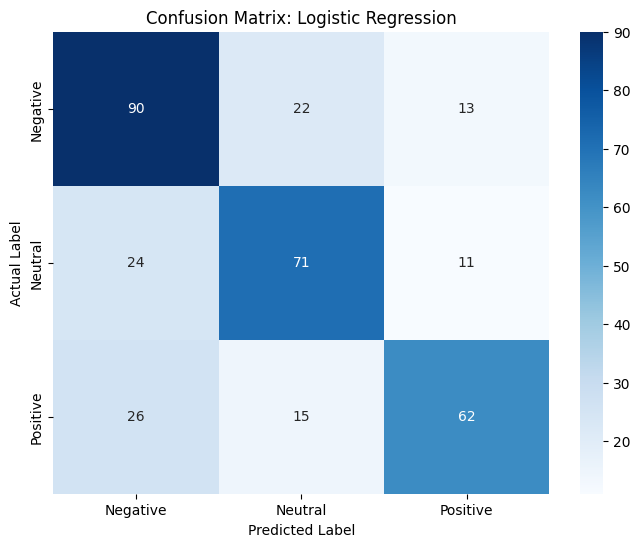
\includegraphics[width=0.49\linewidth]{conf-logistic.png}
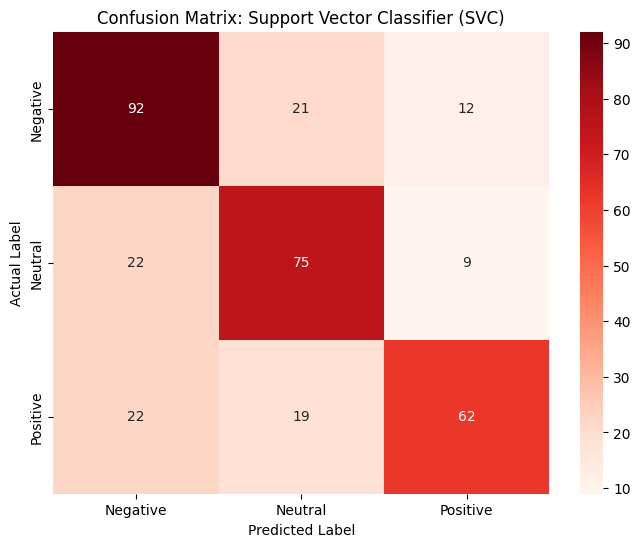
\includegraphics[width=0.49\linewidth]{conf-svc.png}
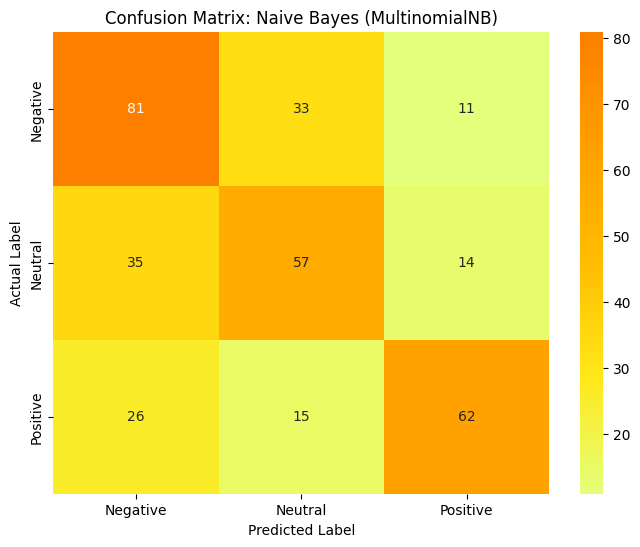
\includegraphics[width=0.49\linewidth]{conf-mult.png}
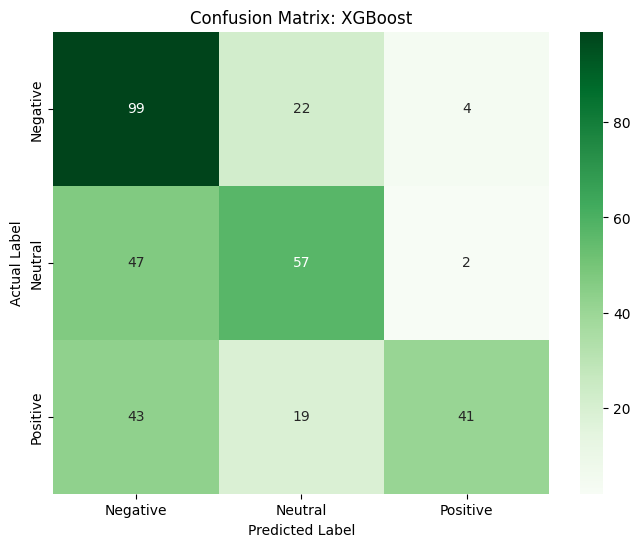
\includegraphics[width=0.49\linewidth]{conf-xgb.png}
\end{figure}
\begin{figure}[H]
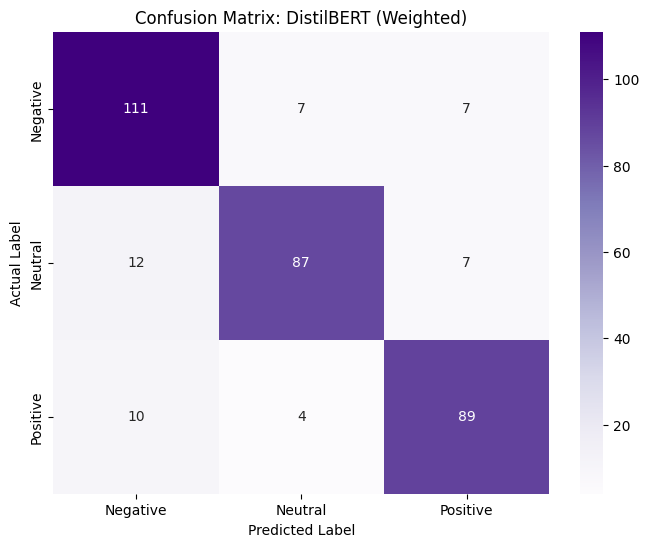
\includegraphics[width=0.49\linewidth]{conf-distil.png}
\caption{Confusion matrices for different models -- rowwise from the top, left-to-right: Logistic Regression, SVC, Naive Bayes (MultinomialNB), XGBoost, and DistilBERT.}
\end{figure}

\begin{figure}[H]
\centering
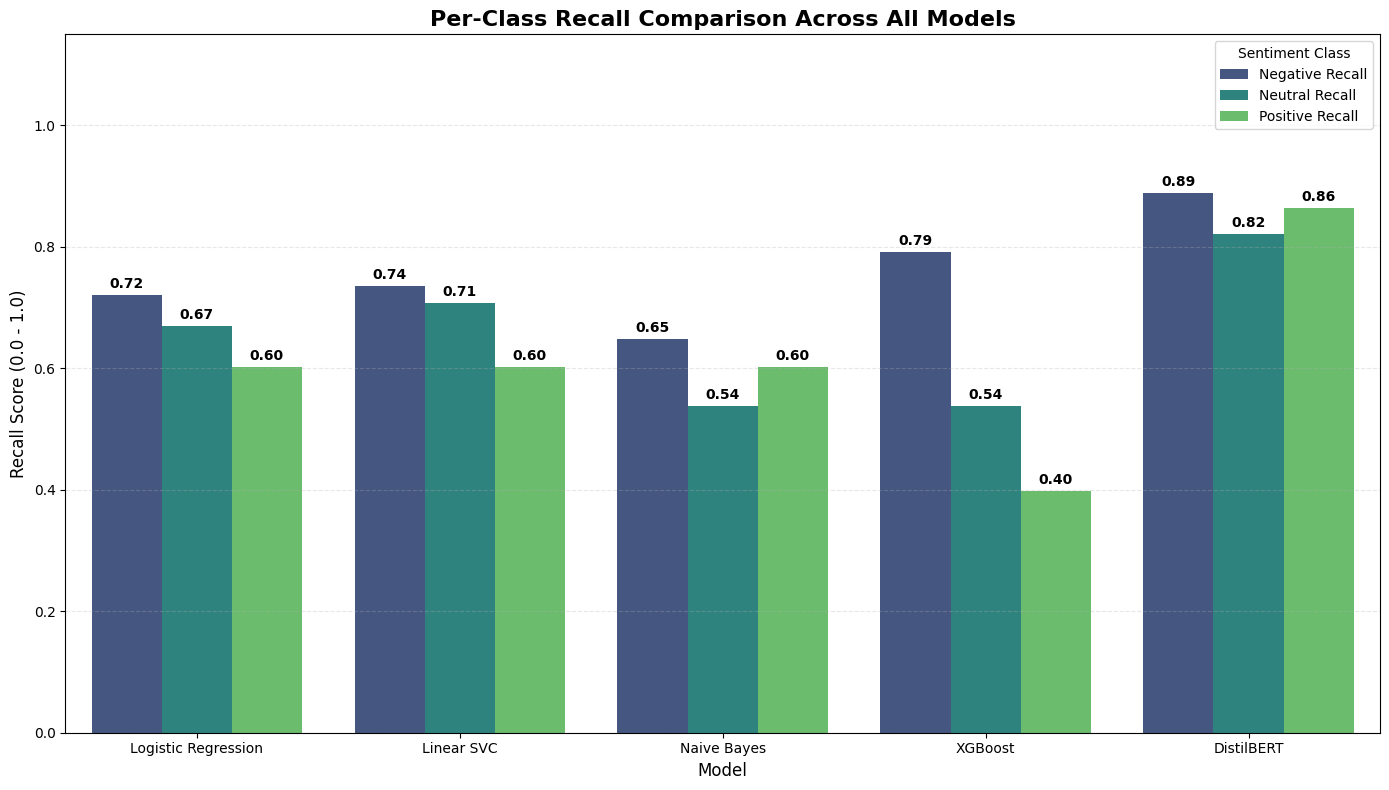
\includegraphics[width=\linewidth]{compare-recall.png}
\caption{Comparison of models' performance -- Classwise Recalls.}
\vspace{1cm}
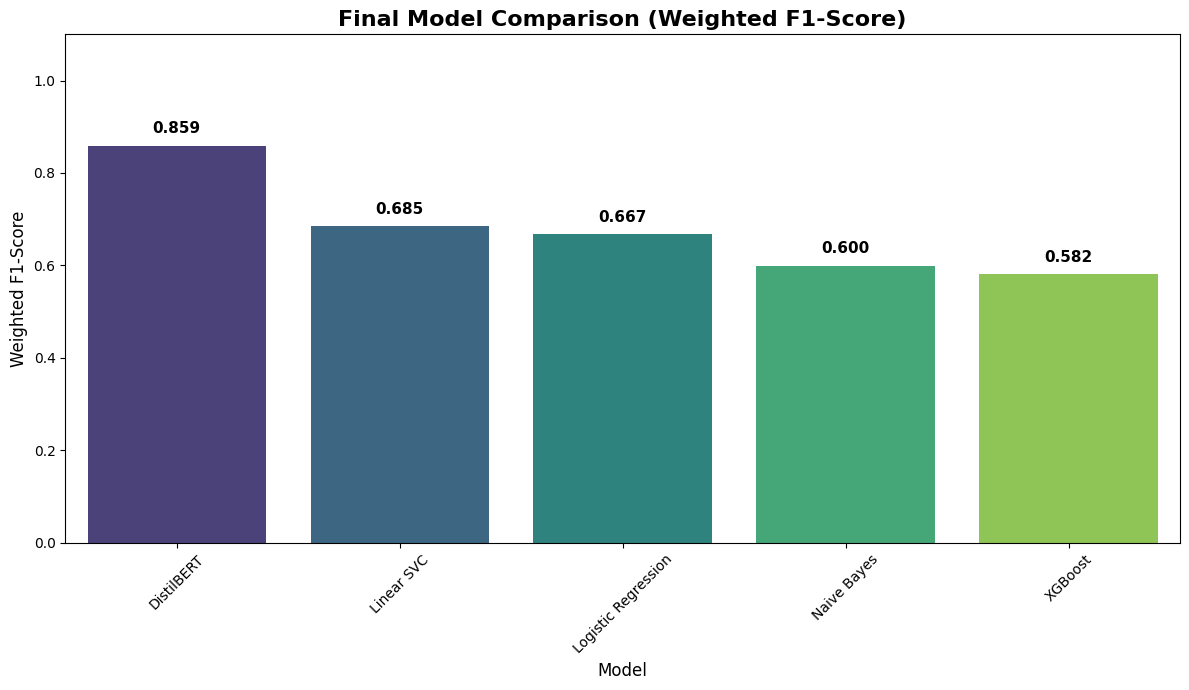
\includegraphics[width=\linewidth]{compare-f1.png}
\caption{Comparison of models' performance -- F1 Scores.}
\end{figure}


% ============================================================
\section{Discussion}
The study highlights the trade-off between interpretability and predictive power. Linear models remain strong baselines for short-text classification, but deep models capture nuanced linguistic signals, especially when comments contain sarcasm, negation, or ambiguous phrasing.

Key observations:
\begin{itemize}
    \item BERT-based models maintain robustness in noisy text.
    \item Preprocessing choices significantly affect classical models but less so for transformers.
\end{itemize}


% ============================================================
\section{Conclusion}
We demonstrated that, for three-class Instagram sentiment classification, transformer-based architectures outperform classical models, though at higher computational cost. SVM remains a strong, fast baseline suitable for deployment in resource-limited settings.

The project highlights the feasibility of automated sentiment classification for informal social-media text and provides a foundation for more advanced multimodal systems.


% ============================================================
\section{Further Work}
\subsection{Context-free Sentiment Analysis}
We examined the feasibility of context-free sentiment analysis, in which comments are classified without relying on accompanying video titles or descriptions. This setup is pragmatically motivated, as Instagram posts often contain minimal or non-informative captions, and recovering context through additional AI pipelines introduces extra computational cost. Our experiments showed that model performances remained largely unchanged under this context-free formulation, although linear models did show a certain amount of improvement.



\begin{figure}[H]
    \centering
    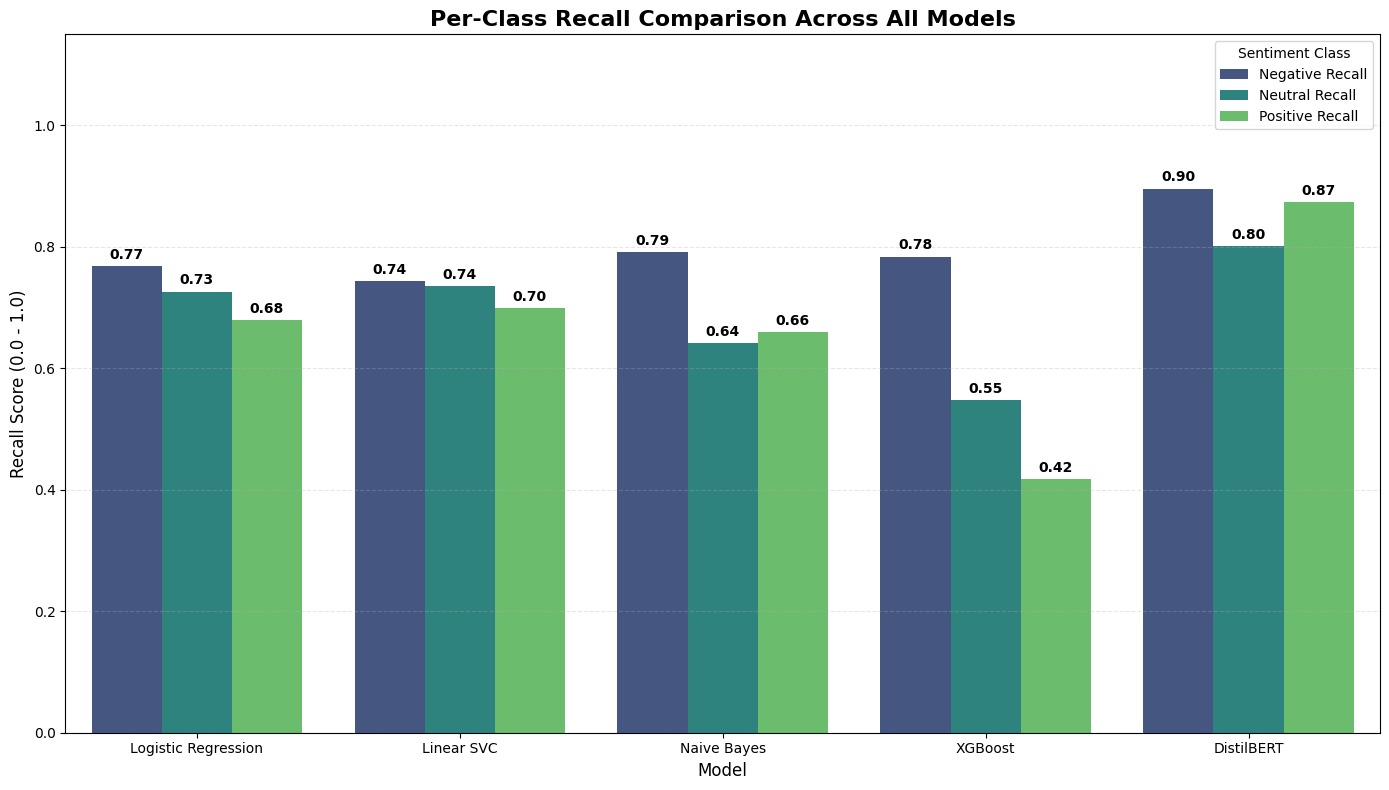
\includegraphics[width=1.1\linewidth]{image1.png}
    \caption{Class recalls of context-free analysis}
    \label{fig:placeholder}
\end{figure}
\begin{figure}[H]
    \centering
    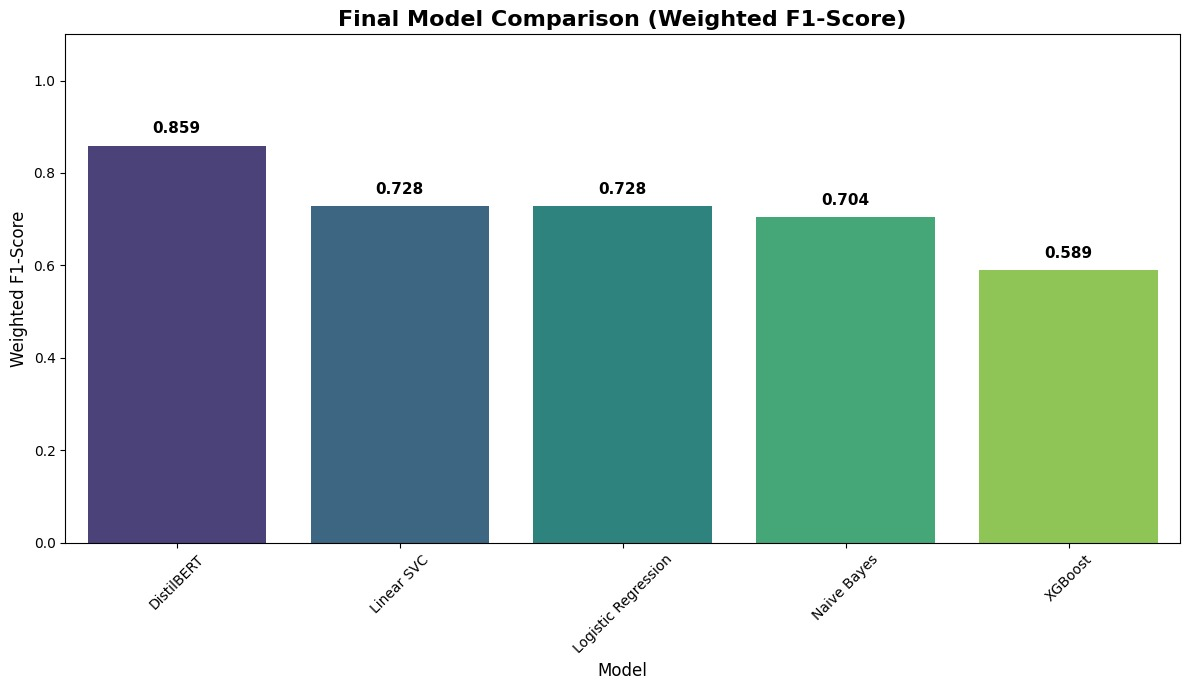
\includegraphics[width=.9\linewidth]{context-free-f1.jpg}
    \caption{F1 scores yielded through context-free analysis.}
\end{figure}


\subsection{Potential extensions}
\begin{itemize}
    \item Domain-adaptive pretraining on Instagram-specific text.
    \item Incorporation of emojis as explicit semantic tokens.
    \item Incorporation of token sequentiality for more precise inference.
    \item Multimodal fusion of text and images for richer sentiment cues.
    \item Continual learning to adapt to evolving slang and usage.
    \item Error analysis on misclassified cases to refine annotation guidelines.
\end{itemize}


% ============================================================
\appendix
\section{Pipeline Summary}
A high-level overview of the modelling pipeline is given below:

\begin{enumerate}
    \item Data ingestion and annotation.
    \item Preprocessing and cleaning.
    \item Model training (LR, SVM, BERT).
    \item Hyperparameter tuning.
    \item Metric computation and model selection.
\end{enumerate}

\end{document}
